\subsection{Compound eyes and the Gabor Super-lens}
When designing optical systems, there usually exists a compromise between two optical properties the field of view (FOV) and resolution. The resolution is related to the ability of the system to minimize aberrations. The field of view is defined as the angular aperture of a frame imaged by the optical system of interest, i.e. the solid angle that spans frame being captured \cite{dobbert2006matchmoving}.\\

Insects such as moths have evolved to have a wide field of view in order to detect predators incoming from various directions. Their eyes are able to achieve this because they are composed of many individual ommatidiums oriented in a semi-sphere as shown in figure \ref{fig:Superposition_Compound_eye}[b]. In this sense, they are termed compound eyes. Compound eyes are natural imaging systems that consist of many independent lenses that act as a system in order to produce images.  An array of the individual lenses is named ommatidium, formally defined as the minimum imaging unit of compound eyes \cite{cheng2019review}. In particular, the field of biological optics distinguishes between three types of compound eyes \cite{volkel2003miniaturized}. These are the apposition \cite{fallah2010mtf}, superposition \cite{greiner2004retinal} and neural superposition compound eyes \cite{frederiksen2008visual}. \\

The design presented in this work closely resembles the refracting superposition compound eye in the sense that all ommatidium focus light into a single point. This type of compound eye are found in insect species such as moths (Figure \ref{fig:Superposition_Compound_eye}).  In particular, this type of compound eyes are characterized for having the best imaging resolution with research reporting resolutions up to ten times higher than that of the apposition compound eye \cite{stollberg2009gabor,kirschfeld1974absolute}. \\

\begin{figure}[H]
    \centering
    \begin{subfigure}[t]{0.48\columnwidth} % Adjust width to fit within column
        \centering
        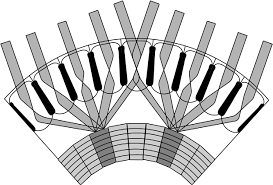
\includegraphics[width=\textwidth]{Figures/refracting superposition compound eye.png}% Ensure correct width
        \label{fig:S_Compound_eye}
    \end{subfigure}
    \hfill
    \begin{subfigure}[t]{0.48\columnwidth} % Adjust width for the second image
        \centering
        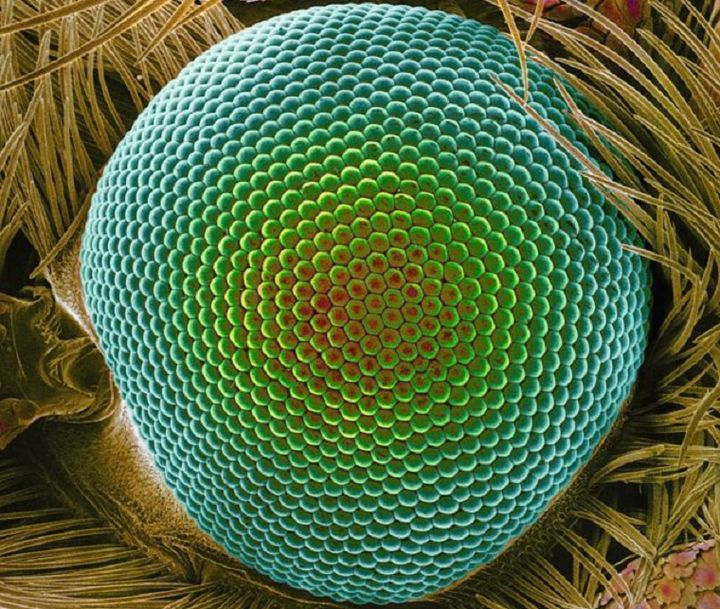
\includegraphics[width=\textwidth]{Figures/Moth_Compound eye.jpg} % Ensure correct width
        \label{fig:Moth}
    \end{subfigure}
    \caption{Transversal view of the superposition compound eye (left); Moth superposition compound eye (right).}
    \label{fig:Superposition_Compound_eye}
\end{figure}



In micro-optics, the practical implementation of superposition compound eyes are termed Gabor super-lenses \cite{stollberg2009gabor} named after Dennis Gabor who in 1940 introduced the concept application for micro-cameras \cite{DGaborSL}. As presented in figure \ref{fig:Gabor design}, the basic Gabor super-lens consists of two micro lenses arrays (MLAs) where the separation is dictated by each layer focal distance. In this sense, the work introduces a Gabor super-lens consisting of three layered micro lens array. In the following section the geometrical considerations are presented.\\ 

\begin{figure}[H]
    \centering
    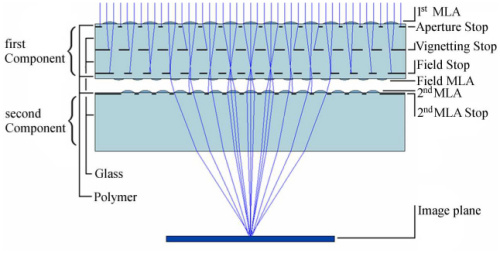
\includegraphics[scale=0.60]{Figures/Gabor-Superlens.jpeg}
    \caption{Gabor super-lens design \cite{stollberg2009gabor} .}
    \label{fig:Gabor design}
\end{figure}

\subsection{Geometric Parameters of the Design}
In this section, a proposal for the Gabor super-lens is presented. The design is built in order to obtain aberration free system, capture a wide field of view and minimize the system´s focal distance. Furthermore, the design consists on a clever arrangement of a three layered ommatidium. Each layer is characterized by its own characteristic curvature that is determined by the focal distance of the structure and the radius of the individual lenses.\\

Consider the structure of the super-lens in the $y-z$ plane with a focal length $f_t$. The lenses in the first layer array (FLA1) have a focal length $f_1$ and a radius $R_1^0 = R_1^n$, where the lower and upper scripts indicate the layer and number of lens inside the array respectively. The center of lenses in FLA1 lie on a vertical line $z=0$ with coordenates $(zc_1^n,yc_1^n)$, where
\begin{equation}
    zc_1^n = 0 \hspace{0.5cm}\&\hspace{0.5cm} yc_1^n = 2nR_1^n ,
\end{equation}
and n is an integer, which has a variation of $-\frac{m-1}{2}\ge n \le \frac{m-1}{2}$. \\

In this case, $m$ is a positive, odd integer that represents the total number of ommatidium arrays. Assuming that rays come from infinity, the rays passing through lenses in FLA1 will focus at the point $P_1=(f_1,yc_1^n)$,as shown in figure \ref{fig:design}. \\

\begin{figure}[H]
    \centering
    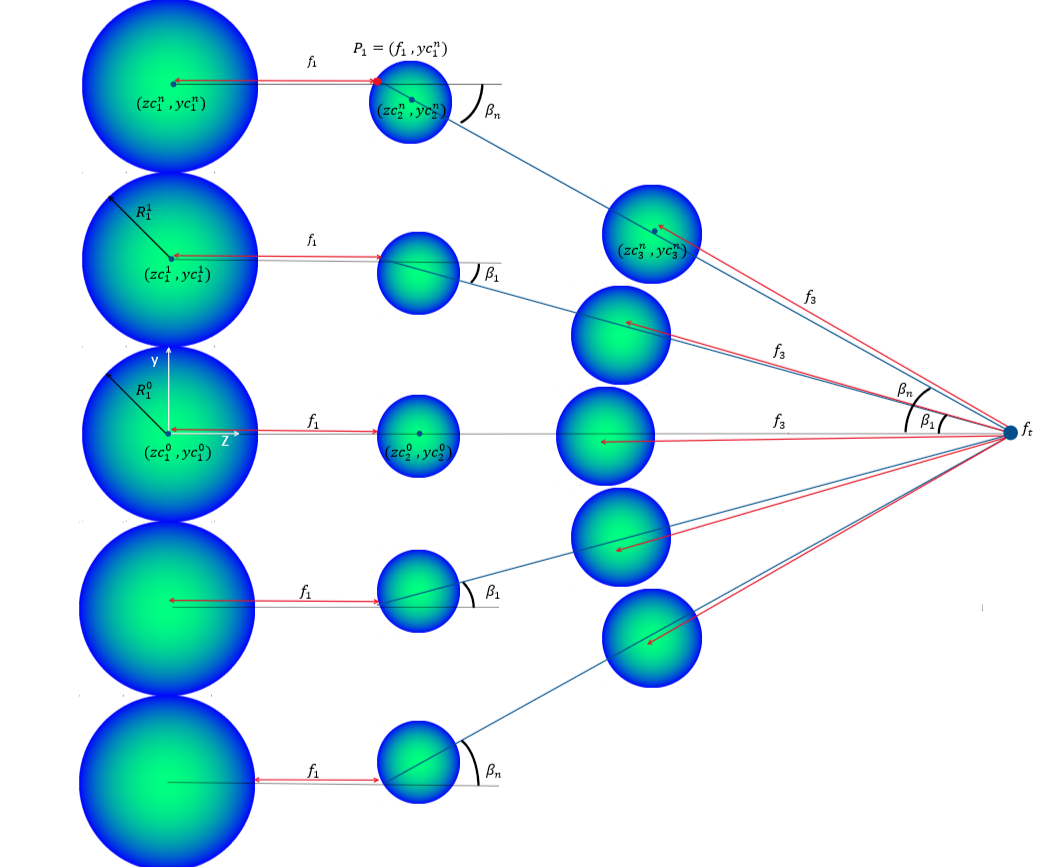
\includegraphics[scale=0.40]{Figures/Superlens_Design_Parameters.png}
    \caption{Super-lens parameters and design.}
    \label{fig:design} 
\end{figure}

The main function of FLA2 is to divert the field from FLA1 in such a way that the center ray will pass through the point $(f_t,0)$. It is known that by placing a source of light on the surface of the Luneburg lens with refractive index $n(r) = \sqrt{2-r^2}$, the field will propagate in the direction given by the angle $\beta_n$, obtaining parallel rays (see figure XXX). The angle $\beta_n$ is given by
\begin{equation}
    \beta_n = arctan(\frac{y_n}{f_1-f_t}).
\end{equation}

In order to ensure the proper diversion, the center of the lenses in FLA2 $(zc_2^n,yc_2^n)$ must be centered in the position

\begin{equation}
\begin{split}
    zc_2^n &= f_1 + R_2^n*cos(\beta_n) \\
    yc_2^n &= yc_1^n - R_2^n*sin(\beta_n),
\end{split}
\end{equation}
where $R_2^n$ is the radius of the Luneburg lenses of FLA2. Note that the centers of these lenses form a curve. \\

The FLA3 must guarantee focus on the point $(f_t,0)$. For this to be possible, the FLA3 lenses must be centered on a point on the line conecting the points $(f_1,yc_1^n)$ and $(f_t,0)$. Their center depends on their focal distance $(f_3)$ and the analytic geometric relation yields
\begin{equation}
\begin{split}
    zc_3^n &= f_t - f_3*cos(\beta_n) \\
    yc_3^n &= f_3*sin(\beta_n). 
    \end{split}
\end{equation}

Note that the radii on FLA3 are not free parameters \footnote{The plural noun results because the each lens is free to have its own radius.}, rather they are restrained by the non linear increment of $\beta_n$ since two lenses cannot overlap. 

\subsection{GRIN Distributions in focal lenses arrays}
Once the geometric parameters of the Gabor lens have been defined, it is important to define the GRIN of the lenses for each FLA. For the FLA1 and FLA3, the GRIN is given by 
\begin{equation}
    n(r) = \left[\frac{(R^2+f^2-\alpha r^2)}{f}\right]^\beta,
\end{equation}

where $f$ is an focal distance factor, $\alpha$ corrects a radial contribution and $beta$ is a non-paraxial correction factor with positive integer values for the 3 parameters. Their value will be obtained in a optimization process. \\

Finally, the lenses in FLA2 are modeled as Luneburg lenses. However a proper normalization factor needs to be introduced for $R_2^n \neq 1$. The normalized GRIN distribution is given by
\begin{equation}
    n(r) = \sqrt{2-\frac{r}{R_2}}.
\end{equation}

